In this section we describe our method in detail. We start by describing the
hypothesis we will evaluate in our paper using MNIST, music and speech data.
\subsection{Hypotheses}

\begin{hyp}[H\ref{hyp:generate}] \label{hyp:generate}
 Generative models can approximate the distribution of real data and hallucinate
 fake data that has some variaety and resembles the real data
\end{hyp}

Although this hypothesis is trivial for experiments that have already been
conducted, it is the first condition for our experiments with music and speech
data. To our knowledge there are no publications where GANs are successful
in hallucinating music and speech data. During out experiments we prove that
this hypothesis is true.

\begin{hyp}[H\ref{hyp:features}] \label{hyp:features}
The real data has useful properties that can be extracted computationally.
\end{hyp}
By useful we refer to properties that are closely related to the real data
itself. For example, computing the distribution MNIST pixel values might be not
useful for assessing drawing quality. However, it might be useful to evaluate
if a random MNIST samples is real or fake data.

\begin{hyp}[H\ref{hyp:visual}] \label{hyp:visual}
The fake data has properties that are hardly noticed with non-computational inspection.
\end{hyp}
Visual inspection of generated samples has become the norm for the evaluation of
samples generated using the GAN framework. We investigate if there are
properties common to all GAN samples or properties that significantly differ
between the real data and the fake data. 
This hypothesis supports the next hypothesis related to adversarial attacks. 

\begin{hyp}[H\ref{hyp:difference}] \label{hyp:difference}
The difference in properties can be used to identify the source (real or fake)
\end{hyp}
The development of generative models for digital media announce the iminent
rise of adversarial attacks. We investigate if these differences can be used to
detect if the data was generated with the GAN framework or is an adversarial
attack.

We call the reader's attention that approximating the distribution over features
computed on the real data does not guarantee that the real data is being
approximated. Formally speaking:
Consider $X \sim Z$, i.e. X distributed as Z, and $f(X) \sim W$, where $f: X
\mapsto Y$.
If $A \sim B$ and $B$ approximates $Z$, then $f(A) \sim D$ must also approximate $W$.
However, a distribution that approximates $W$ is not guaranteed to approximate
$Z$.

\subsection{Learning properties}
In this subsection, we describe the properties that we mine from data. They
comprise of properties that are perceptually related with the image and
properties that are not perceptually related but that can be used to identify
the source of the image. Consider the single channel image $I$ with dimensions 
$R$ by $C$, where $I_{r, c}$ is the pixel intensity of the pixel at row $r$ and column $c$

\subsubsection{Summary Statistics}
Consists of the distribution of mean, standard
deviation, kurtosis and skewness feature values over all images. It is applied
to pixel intentisy and some features described below.

\subsubsection{Spectral Moments}
The spectral centroid is a feature commonly used in the audio domain, where it
represents the barycenter of the spetrum. Given an image, for each column we transform the
pixel values into probabilities by normalizing them by the column sum, after which we
take the expected row value. Given one image column, we define $r$ as the pixel
intensity at row $r$, and 

\begin{equation}
    p(r) = \frac{r}{\sum_{r in R}r}
\end{equation}

From these definitions, it immediately follows that the first, second, third and fourth moments
can be described as follows: 
\begin{equation}
    \mu = \int rp(r) \partial r
\end{equation}

\begin{equation}
    \sigma^2 = \int (r - \mu)^2 p(r) dr
\end{equation}

\begin{equation}
    \gamma_1 = \frac{\int (r - \mu)^3 p(r) dr}{\sigma^3}
\end{equation}

\begin{equation}
    \gamma_2 = \frac{\int (r - \mu)^4 p(r) dr}{\sigma^4}
\end{equation}

Figure~\ref{fig:mnist_centroids} shows the spectral centroid computed
on sample of MNIST training data.

\begin{figure}[!h]
  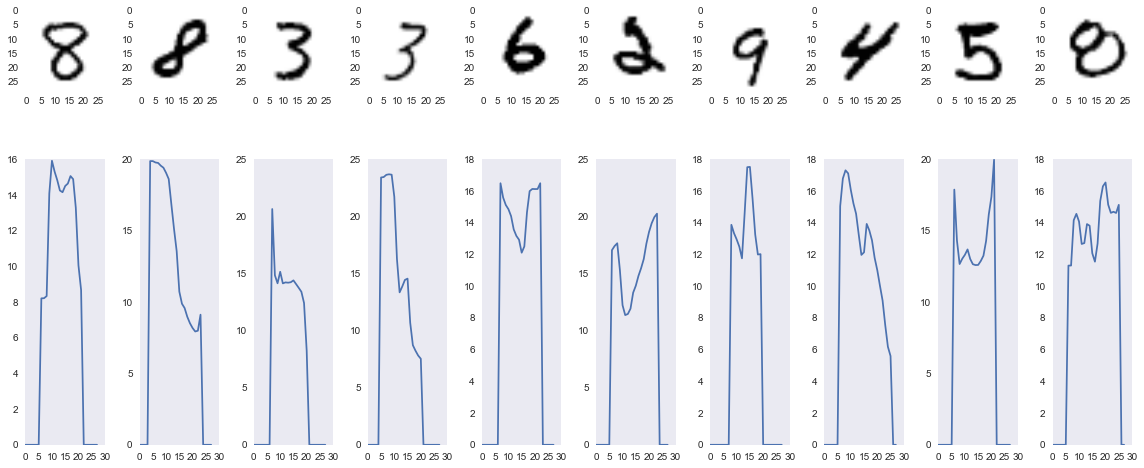
\includegraphics[width=\linewidth]{mnist_centroids.png}
  \caption{}
  \label{fig:mnist_centroids}
\end{figure}

\subsubsection{Spectral Slope}
Is computed by linear regression on the sepectral centroid with window of size
7. Figure~\ref{fig:mnist_spectral_slope} shows these features computed on a
sample of MNIST training data.

\begin{figure}[!h]
  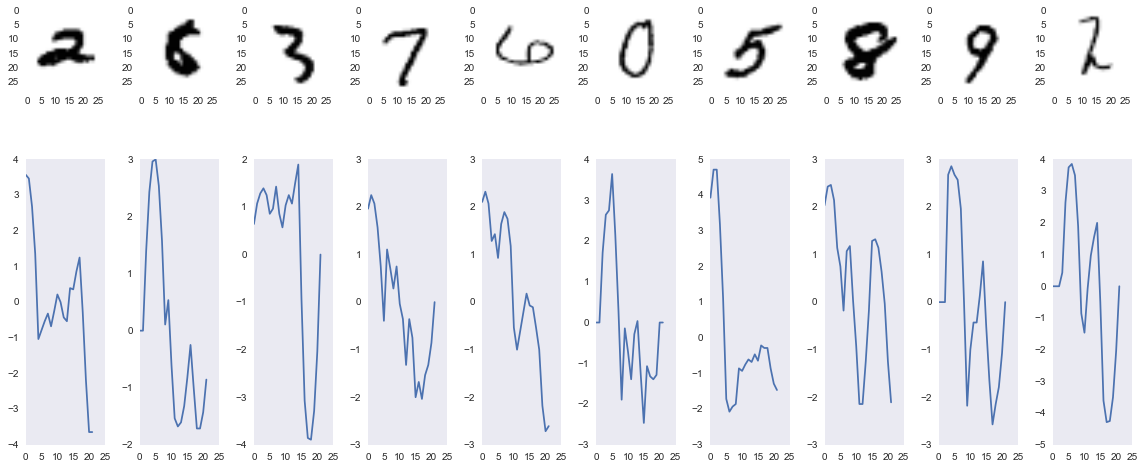
\includegraphics[width=\linewidth]{mnist_spectral_slope.png}
  \caption{}
  \label{fig:mnist_spectral_slope}
\end{figure}

\subsubsection{Transition Matrix}
Transition matrix is computed only for chromagram representations of piano
rolls. \\
Equation

\subsection{Distance Measures}
We use the Kolgomorov-Smirnov Two Samples Test\\
Equation

We use the Jensen-Shannong Divergence\\
Equation

\subsection{Generative Adversarial Networks}
We investigate the DCGAN architecture under LSGAN, WGAN, IWGAN objective
functions.
